\lstset{style=fsharpstyle}

\section{Используемые технологии}
\label{sec:practice:technology_used}
Выбор технологий является важным предварительным этапом разработки сложных информационных систем.
Платформа и язык программирования, на котором будет реализована система, заслуживает большого внимания, так как исследования показали, что выбор языка программирования влияет на производительность труда программистов и качество создаваемого ими кода.

Ниже перечислены некоторые факторы, повлиявшие на выбор технологий:
\begin{itemize}
\item Разрабатываемое ПО должно иметь возможность запускаться под платформами Windows(7,8,10);
\item Дальнейшей поддержкой проекта, возможно, будут заниматься разработчики, не принимавшие участие в выпуске первой версии;
\item Имеющийся разработчик имеет опыт работы с объекто"=ориентированными языками программирования.
\end{itemize}

Основываясь на опыте работы имеющихся программистов разрабатывать ПО целесообразно с помощью языка С++.
Приняв во внимание необходимость обеспечения доступности дальнейшей поддержки ПО, возможно, другой командой программистов, необходимость работы с различными ОС, целесообразно не использовать малоизвестные и сложные языки программирования.
Так как при разработке програмного средства будет использоваться симулятор DRAM, написанный на С++, целесообразно выбрать именно этот язык для создания внешней среды для этого симулятора.
Таким образом, с учетом вышеперечисленных факторов, целесообразно остановить выбор на следующих технологиях:
\begin{itemize}
  \item операционные системы: семейство Windows(7,8,10);
  \item язык программирования С++.
\end{itemize}
Для реализации поставленной задачи предпочительно использовать стандартную библиотеку STL без использования сторонних библиотек для обеспечения простой компиляции проекта под любой операционной системой.
Высокий уровень абстракции языка, полноценные механизмы ООП, большое количество контейнеров и алгоритмов библиотеки STL позволяют наиболее просто и <<красиво>> решить поставленную задачу.
Разрабатываемое программное обеспечение в некоторой степени использует данное преимущество языка.

Далее проводится характеристика используемых технологий и языка программирования более подробно.

\subsection{Язык программирования С++}
\label{sub:practice:cpp_overview}
С++ - компилируемый, статически типизированный язык программирования общего назначения. Синтаксис C++ унаследован от языка C. Одним из принципов разработки было сохранение совместимости с C. Тем не менее, C++ не является в строгом смысле надмножеством C; множество программ, которые могут одинаково успешно транслироваться как компиляторами C, так и компиляторами C++, довольно велико, но не включает все возможные программы на C.

Язык поддерживает такие парадигмы программирования, как процедурное программирование, объектно-ориентированное программирование, обобщённое программирование, обеспечивает модульность, раздельную компиляцию, обработку исключений, абстракцию данных, объявление типов (классов) объектов, виртуальные функции. Стандартная библиотека включает, в том числе, общеупотребительные контейнеры и алгоритмы. C++ сочетает свойства как высокоуровневых, так и низкоуровневых языков. В сравнении с его предшественником — языком C, — наибольшее внимание уделено поддержке объектно-ориентированного и обобщённого программирования \cite{cpp_book}.

C++ широко используется для разработки программного обеспечения, являясь одним из самых популярных языков программирования. Область его применения включает создание операционных систем, разнообразных прикладных программ, драйверов устройств, приложений для встраиваемых систем, высокопроизводительных серверов, а также развлекательных приложений (игр). Существует множество реализаций языка C++, как бесплатных, так и коммерческих и для различных платформ. Например, на платформе x86 это GCC, Visual C++, Intel C++ Compiler, Embarcadero (Borland) C++ Builder и другие. C++ оказал огромное влияние на другие языки программирования, в первую очередь на Java и \csharp{}.

Главное нововведение C++ - механизм классов, дающий возможность определять и использовать новые типы данных. Программист описывает внутреннее представление объекта класса и набор функций-методов для доступа к этому представлению. Одной из заветных целей при создании C++ было стремление увеличить процент повторного использования уже написанного кода. Концепция классов предлагала для этого механизм наследования. Наследование позволяет создавать новые (производные) классы с расширенным представлением и модифицированными методами, не затрагивая при этом скомпилированный код исходных (базовых) классов. Вместе с тем наследование обеспечивает один из механизмов реализации полиморфизма - базовой концепции объектно-ориентированного программирования, согласно которой, для выполнения однотипной обработки разных типов данных может использоваться один и тот же код. Собственно, полиморфизм - тоже один из методов обеспечения повторного использования кода \cite{cpp_book_two}.

Введение классов не исчерпывает всех новаций языка C++. В нем реализованы полноценный механизм структурной обработки исключений, отсутствие которого в С значительно затрудняло написание надежных программ, механизм шаблонов - изощренный механизм макрогенерации, глубоко встроенный в язык, открывающий еще один путь к повторной используемости кода, и многое другое.

Таким образом, генеральная линия развития языка была направлена на расширение его возможностей путем введения новых высокоуровневых конструкций при сохранении сколь возможно полной совместимости с ANSI С. Конечно, борьба за повышение уровня языка шла и на втором фронте - те же классы позволяют при грамотном подходе упрятывать низкоуровневые операции, так что программист фактически перестает непосредственно работать с памятью и системно-зависимыми сущностями.

\subsection{Симуляторы ДОЗУ}
\label{sub:domain:simulators}
Для моделирования процессов оперативной памяти используется множество симуляторов, от упрощенных моделей, которые лишь регулируют временные задержки и пропускную способность доступа к памяти, и до детализированных симуляторов, которые могут точно отразить сложное поведение современных систем памяти. К сожалению, в открытом доступе находится малая их часть. В этом разделе будут рассмотрены и сравнены некоторые симуляторы, информация о которых имеется в открытых источниках.

\subsubsection{DRAMSim2}
\label{sub:domain:simulators:dramsim2}
Одним из популярных симуляторов памяти является DRAMSim2, разработанный в университете Мэриленд, США. 
DRAMSim2 – это потактовый симулятор оперативной памяти, реализованный на языке С++ как объектно-ориентированная модель DDR2/3 памяти. Помимо прочего данный симулятор обеспечивает надежный инструмент для визуализации и сравнения влияния системных параметров памяти на ключевые метрики производительности, такие как пропускная способность, временные задержки и потребляемую мощность \cite{dramsim2_article}.

Ядро симулятора заключено в единый объект, который называется MemorySystem. Он состоит из двух компонент: контроллера памяти и ОЗУ. Диаграмма главных компонентов симулятора DRAMSim2 и их связей изображена на рисунке~\ref{fig:domain:simulators:dramsim2:dramsim2_component}. 

\begin{figure}[ht]
\centering
  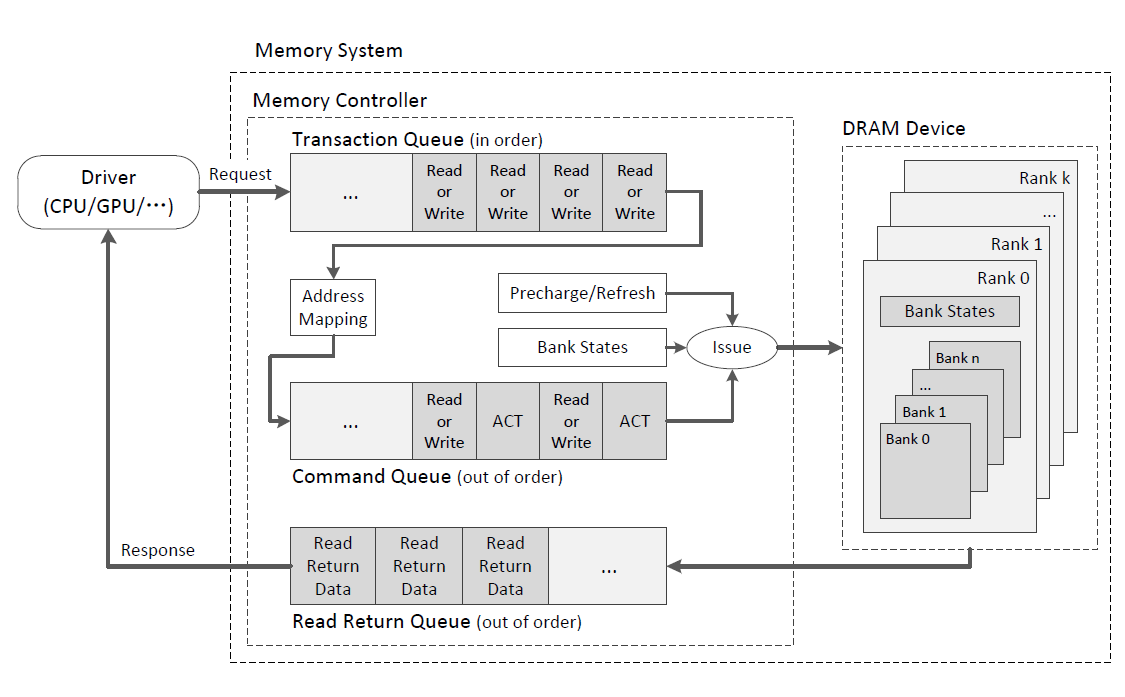
\includegraphics[scale=0.4]{a_dramsim2_components.png}  
  \caption{Диаграмма компонентов симулятора DRAMSim2}
  \label{fig:domain:simulators:dramsim2:dramsim2_component}
\end{figure}

Для объекта MemorySystem необходимо наличие двух ini-файлов: для инициализации системы в целом и для описания ОЗУ. Файл инициализации ОЗУ содержит описание параметров конкретного устройства, таких как временные ограничения и параметры энергопотребления устройства. Значения этих параметров можно найти в справочных данных, предоставляемых производителями ОЗУ.

Пакет DRAMSim2 содержит несколько ini-файлов для устройств Micron DDR2/3 различного объёма и скорости. Ini-файл системы содержит параметры, независящие от конкретного типа ОЗУ. Они включают в себя такие параметры, как схемы отображения адресов, опции отладки, структура очереди контроллера памяти и другие детали симуляции.

После создания объекта  MemorySystem код драйвера памяти должен зарегистрировать функции обратного вызова, чтобы получать уведомления о выполнении запросов. На этом этапе инициализация симулятора завершена. Код драйвера должен вызывать специальную функцию для каждого системного такта, а также другую функцию, для добавления запроса к памяти. По окончании обработки запроса симулятор информирует драйвер о выполненном действии, вызывая зарегистрированную функцию обратного вызова \cite{dramsim2_manual}.

Поскольку вся логика взаимодействия с симулятором заключена в простом интерфейсе с минимальным количеством функций, симулятор  легко внедрить в любую систему, будь то простой драйвер или потактовый симулятор ЦП, такой как MARSSx86. 
DRAMSim2 может быть скомпилирован как автономный исполняемый модуль, либо же в качестве библиотеки. Соответственно симулятор работает в двух режимах : автономном и встроенном в другую систему. В автономном режиме симулятор считывает список команд из trace-файла, хранящегося на диске. Во встроенном режиме симулятор предоставляет базовую функциональность для создания объекта системы памяти и добавления запросов к нему. 

DRAMSim2 не использует никаких сторонних библиотек, кроме стандартной библиотеки C++ STL. Благодаря этому симулятор легко скомпилировать под любой операционной системой, на которой установлен компилятор GNU C++. Для запуска симулятора под OС Windows потребуется Cygwin.

Поскольку производители отказываются публиковать детали работы их контроллеров памяти, DRAMSim2 моделирует современные DDR2/3 контроллеры в общем виде. Запросы от драйвера (любой модуль, который выдаёт запросы, например центральный процессор) накапливаются в очереди транзакций в порядке их выполнения.  Эти транзакции преобразуются в команды ОЗУ и направляются в очередь команд, а затем выдаются запоминающему устройству. Контроллер памяти отслеживает состояние каждого банка памяти, на основе чего определяет, какой запрос должен быть передан ОЗУ следующим. Взаимодействие драйвера, контроллера памяти и DRAM отображено на рисунке~\ref{fig:domain:simulators:dramsim2:dramsim2_component}. Выдача запросов в случайном порядке помогает оптимизировать использование банка и тем самым повысить пропускную способность памяти и уменьшить задержки.

После получения устройством DRAM команды и данных от контроллера памяти, список состояний банков используется для проверки ошибок, чтобы убедиться, что время полученной команды верное. 

В дополнение к моделированию изменения состояния системы во время операций чтения и записи, контроллер памяти DRAMSim2 так же моделирует эффект восстановления памяти ОЗУ. Моделирование регенерации памяти имеет важное значение, так как операции восстановления являются основным источником задержек при выполнении запросов к памяти. Запросы чтения, поступившие во время восстановления памяти, должны ожидать обработки намного дольше, чем другие запросы. 

Достоинством симулятора DRAMSim2 является простой интерфейс, общедоступный исходный код, который можно скачать с сайта GitHub.com, подробная документация, наличие готовых конфигурационных файлов для различных типов памяти. Симулятор легко скомпилировать под любой операционной системой, при этом не требуется инсталляция дополнительных библиотек.  В качестве серьёзного недостатка является отсутствие в бесплатной версии симулятора возможности записи и считывания данных, но относительная простота кода и грамотная архитектура системы позволяет программисту доработать этот момент.  

\subsubsection{Ramulator}
\label{sub:domain:simulators:ramulator}
Ramulator – это быстрый, потактовый DRAM симулятор, целью создания которого была потребность в расширяемом симуляторе, который может быль легко модифицирован под любой стандарт памяти, чтобы иметь представление о достоинствах современных DRAM \cite{ramulator_manual}.

В основе Ramulator лежит обобщённый шаблон для моделирования систем DRAM, который позже конкретизируется под определённый стандарт памяти. Благодаря такому гибкому дизайну симулятор может обеспечить поддержку широкого спектра стандартов DRAM: DDR3/4, LPDDR3/4, GDDR5, WIO1/2, HBM, а также академических стандартов(SALP, AL-DRAM, TLDRAM, RowClone, and SARP).  Важно заметить, что данный симулятор не жертвует скоростью памяти для обеспечения такой расширяемости и гибкости. 

Ramulator основывается на важном наблюдении: любая DRAM может быть представлена в виде иерархии конечных автоматов, где поведение каждого автомата, как и иерархии в целом, диктуется стандартами DRAM.
Из любого предоставленного стандарта DRAM симулятор извлекает полную спецификацию для иерархии конечных автоматов и их поведения, которую затем объединяет в единый класс(например, DDR3.h/cpp). Вследствие этого симулятор легко переконфигурировать под другой стандарт памяти, что не требует изменений в коде.

В листинге ~\ref{lst:domain:simulators:ramulator:code} представлен сласс DRAM, который является обобщенным шаблоном для построения иерархии (дерева) конечных автоматов (узлов). Экземпляр класса DRAM  - это один из узлов в дереве, который будет заключать в себе конкретную реализацию стандарта DRAM (DRAM<DDR3>).

\begin{lstlisting}[style=cplusplusstyle, caption={Метод записи конкретных бит в слове}, label=lst:domain:simulators:ramulator:code]
// DRAM.h
template <typename T>
class DRAM {
  DRAM<T>* parent;
  vector<DRAM<T>*> children;
  T::Level level;
  int index;
  //more code...
};

// DDR3.h/cpp
class DDR3 {
  enum class Level {
    Channel,
    Rank,
    Bank,
    Row,
    Column,
    MAX
  };

  //more code...
};
\end{lstlisting}

На рисунке ~\ref{fig:domain:simulators:ramulator:tree} представлено полностью реализованное дерево, состоящее из узлов различного уровня: от канала до банка. Вместо того, чтобы создавать отдельный класс для каждого уровня (DDR3 Channel, DDR3 Rank, DDR3 Bank), Ramulator просто представляет каждый уровень как очередное свойство узла дерева. Это свойство может быть легко переназначено для адаптации иерархий под различные уровни. Ramulator так же предоставляет контроллер памяти, который взаимодействует с деревом через его корень. Каждый раз, когда контроллер памяти инициирует запрос или операцию, производится обход дерева, затрагивающий только необходимые узлы во время выполнения процесса.

\begin{figure}[ht]
\centering
  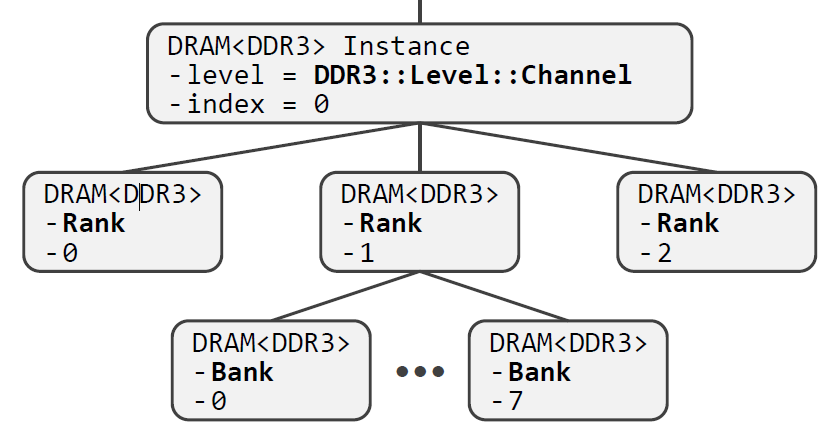
\includegraphics[scale=0.5]{a_ramulator_tree.png}  
  \caption{Дерево конечных автоматов памяти DDR3}
  \label{fig:domain:simulators:ramulator:tree}
\end{figure}

Система конечных автоматов подразумевает набор состояний, переход между которыми осуществляется под внешним воздействием. Конечный автомат рассматриваемого симулятора хранит в себе текущее состояние, которое может принимать одно из значений, определяемых в классе конкретного вида памяти (например, DDR3). Узел может переходить из одного состояния в другое при получении одной из команд, которые так же определяются классом симулируемой памяти. Так же узел хранит в себе таблицу временных параметров, по которой определяется ближайшее время, через которое узел сможет принять ту или иную команду. Цель этой таблицы – предотвратить преждевременный переход узла из одного состояния в другое.  У каждого узла в дереве есть 3 функции: decode, check и update. Команда, поступившая к конкретному узлу, должна декодироваться. Функция decode распознаёт команду и проверяет возможность её выполнения, основываясь на статусе узла. Например, команда чтения не может быть выполнена, если rank отключен или bank закрыт. Для данной команды и адреса функция decode вернёт команду, которая должна быть выполнена перед командой чтения.  Даже если нет команд, которые должны быть предварительно выполнены перед операцией, это не означает, что поступившая команда может выполняться тут же. Например, bank может быть не готов к чтению, если он был активирован недавно. Для этих целей функция check сообщает, можно ли выполнить команду прямо сейчас (на текущем цикле). Если функция check разрешила выполнение команды, то контроллер памяти выполняет ее. Функция update в зависимости от команды модифицирует статус узла и его временные параметры в таблице.

Кроме того Ramulator поддерживает унифицированный контроллер памяти, который совместим со всеми стандартами DRAM(поддерживаемых в симуляторе). Контроллер памяти содержит три очереди запросов к памяти:  чтение, запись и техническое обслуживание. В то время, как очереди чтения/записи наполняются запросами, поступившими от внешнего источника команд (trace-файл с командами чтения и записи), очередь технического обслуживания узлов наполняется другим видом команд (обновление, отключение питания, автообновление), генерируемых внутри контроллера памяти, когда они необходимы. Для обработки запросов трёх очередей контроллер памяти взаимодействует с иерархическим деревом DRAM используя три функции узла, описанные выше.  

Таким образом Ramulator представляет собой расширяемый DRAM симулятор, обеспечивающий потактовую модель широкого разнообразия стандартов: DDR3/4, LPDDR3/4, GDDR5, WIO1/2, HBM, SALP, ALDRAM, TL-DRAM, RowClone, and SARP. Модульная архитектура системы позволяет легко дополнять симулятор новыми стандартами. Для некоторых стандартов Ramulator способен предоставлять отчеты по энергопотреблению. Ramulator оснащен простым контроллером памяти, представляющим из себя внешнее API для отправки и получения запросов памяти. Симулятор доступен в двух различных форматах : для автономного использования и для встроенного в систему режима. Для компиляции симулятора требуется компилятор GNU C++ и библиотека clang++. Из-за использования дополнительной библиотеки могут возникнуть трудности при компиляции проекта в операционной системе Windows. В бесплатной версии симулятора отсутствует возможность реального хранения данных.

\subsubsection{Обоснование выбора симулятора DRAM}
\label{sub:domain:simulators:simulator_choice}
Среди прочих симуляторов, информация о которых есть в открытом доступе, можно отметить еще несколько симуляторов. 

DrSim – потактовый симулятор DRAM памяти. Поддерживает стандарты памяти DDR2, DDR3 и LPDDR2. Написан на языке С++. Для компиляции потребуется GNU C++ и GNU Make. В целом этот симулятор очень напоминает DRAMSim2. Он так же работает в двух режимах: автономном и встроенном. В конфигурационных файлах задаются параметры для конкретного типа DRAM, а также основные параметры для системы в целом. В режиме атвономной работы команды считываются из trace-файла, результаты выполнения выводятся на консоль. Во встроенном режиме внешней системе нужно выполнять роль генератора тактов для памяти, а также отправлять запросы. По завершении выполнения запроса вызывается функция обратного вызова, чтобы позволить пользователю увидеть результаты выполнения команды \cite{drsim_manual}.

USIMM – симулятор DRAM, поддерживающий стандарт DDR3. Симулятор написан на языке С, без использования дополнительных библиотек. Главный модуль симулятора запускает цикл, в котором он получает команду из очереди запросов и запускает функцию updateMemory. Эту функцию реализует контроллер памяти, который проверяет временные параметры DRAM, чтобы определить, какие команды могут быть выполнены на данном цикле. Пользователь должен предоставить функцию scheduler, которая будет выдавать команды для каналов в каждый цикл работы памяти. В конфигурационных файлах описываются параметры для симулируемой памяти \cite{usimm_manual}. 

Среди рассмотренных симуляторов Ramulator является наиболее гибкой и хорошо спроектированной моделью динамической памяти. Однако при попытке компиляции проекта под ОС Windows возникли проблемы с библиотекой clang++. Данный симулятор поддерживает широкий круг стандартов памяти, однако в рамках задачи дипломного проекта такой широты не требуется. Симулятор DRAMSim2 является относительно простым и небольшим проектом, который легко скомпилировать под любой операционной системой, при этом не требуется инсталляция дополнительных библиотек. Простой интерфейс позволяет легко встраивать симулятор в другие системы. Симуляторы DrSim и USIMM во многом уступают симулятору DRAMSim2. Как по наличию скромной документации, так и по грамотности построения структуры исходного кода и удобству использования. В открытом доступе отсутствуют симуляторы с возможностью хранения реальных данных, вследствие чего симулятор DRAMSim2 вполне подойдёт для дополнительных модификаций и адаптаций под текущую задачу проекта. 